% ECE578 Project
% Bliss Brass, Kai Brooks, Tyler Hull, Mikhail Mayers, Roman Minko
% Fall 2019

% Document settings ------------------------------------------------
\documentclass[a4paper,12pt]{article}

\newcommand{\figOverlay}{\put(34,10){\color{black!50} \figWatermark}} % Figure overlay settings
\newcommand{\figWatermark}{}%\small Brooks \today} 		% Figure overlay text
\newcommand{\figHere}{\begin{overpic}[percent,scale=0.3]}	% Settings for all figures
\newcommand{\figHereB}{\begin{overpic}[percent,scale=2]}	% Settings for all figures
\newcommand{\figHereC}{\begin{overpic}[percent,scale=0.5]}	% Settings for all figures

\newcommand{\figHereD}{\begin{overpic}[percent,scale=0.7]}	% Settings for all figures

\newcommand{\authorname}{Brass, Brooks, Hull, Mayers, Minko}
\newcommand{\classnumber}{ECE578}
\newcommand{\projectname}{Mice and Cheese}


\newcommand{\robotServerName}{Python code for robot server}

% Packages ------------------------------------------------

\usepackage[USenglish]{babel} 	% American English
\usepackage{blindtext}			% Generate latin crap
\usepackage[yyyymmdd]{datetime} % Sets date format to ISO 8601 standard
\renewcommand{\dateseparator}{-}% Sets date format to ISO 8601 standard

\usepackage{graphicx}			% Image importing and display
\graphicspath{ {images/} }		% Path to image folder
\usepackage{xcolor}				% Allows normal color words
\usepackage{color, colortbl}


\usepackage{float}				% Adds 'H' for figure placement location
\usepackage{enumitem}			% Use for QandA environment
\usepackage{booktabs}			% Merging columns in tables

\usepackage[nostamp]{draftwatermark}	% use [nostamp] when finished, [firstpage] otherwise
\SetWatermarkText{DRAFT}
\SetWatermarkColor{red!50}
\SetWatermarkScale{3}


\usepackage{overpic}				% Puts text over figures
\usepackage[american]{circuitikz}	% American-style circuit diagrams

\usepackage{amsmath}				% Multi-line equations
\usepackage{caption}				% Equation caption formatting
\usepackage{physics}				% Easier derivatives
\usepackage{gensymb}				% Enable \degree for degree symbol
\usepackage{siunitx}				% SI units

\usepackage{hyperref}				% makes links
\usepackage[normalem]{ulem}			% adds strikethrough

\usepackage{listings}				% inline code

\usepackage{array}					% Used for centering tabular data
\newcolumntype{M}[1]{>{\centering\arraybackslash}p{#1}} % The actual centered column format

\usepackage{listings} %For code in appendix

% background image for the first page
\usepackage{eso-pic}
\newcommand\BackgroundPic{%
\put(0,0){%
\parbox[b][\paperheight]{\paperwidth}{%
\vfill
\centering
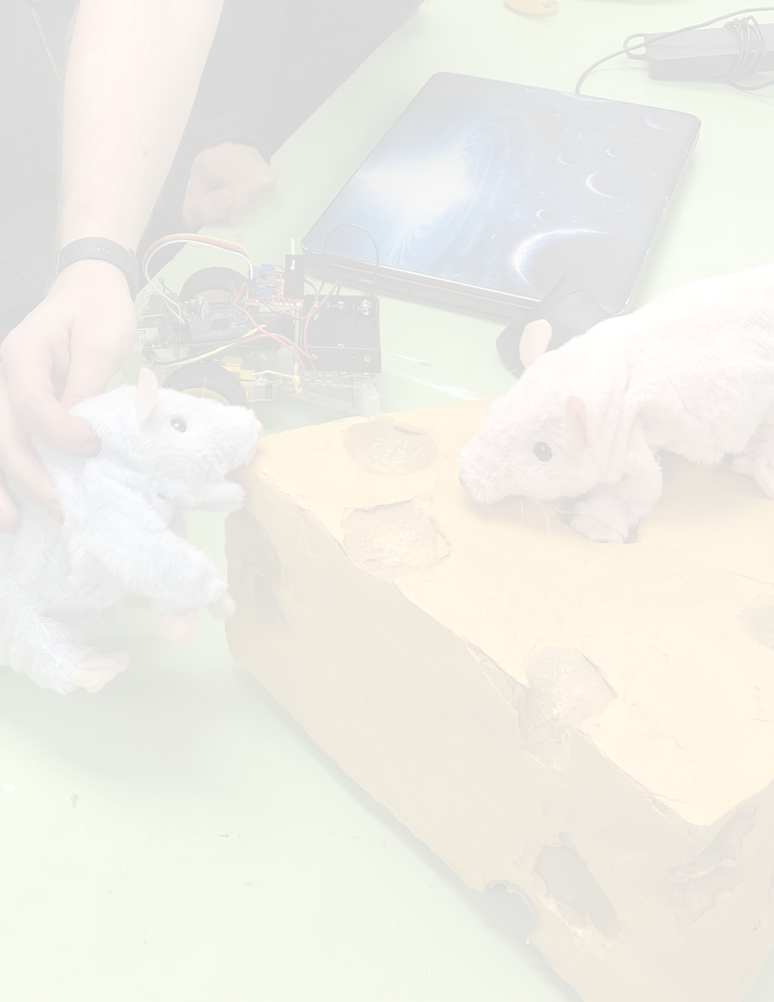
\includegraphics[width=\paperwidth,height=\paperheight]{images/bg.png}%
\vfill
}}}

\definecolor{mymauve}{rgb}{0.58,0,0.82}
\definecolor{mygreen}{rgb}{0,0.6,0}
\definecolor{mygray}{rgb}{0.5,0.5,0.5}
\definecolor{ltgray}{rgb}{0.937, 0.937, 0.956}	% Divide standard RGB values by 255 for some reason 

% PSU colors
\definecolor{PSUgreen}{RGB}{106,127,16}
\definecolor{PSUltgreen}{RGB}{168,180,0}
\definecolor{PSUblue}{RGB}{0,117,154}
\definecolor{PSUltblue}{RGB}{161,216,224}
\definecolor{PSUgray}{RGB}{71,67,52}
\definecolor{PSUbrown}{RGB}{96,53,29}
\definecolor{PSUsienna}{RGB}{163,63,31}
\definecolor{PSUred}{RGB}{210,73,42}
\definecolor{PSUorange}{RGB}{220,155,50}
\definecolor{PSUyellow}{RGB}{230,220,143}
\definecolor{PSUtan}{RGB}{232,221,162}
\definecolor{PSUpurple}{RGB}{101,3,96}


\newenvironment{QandA}
	{\begin{enumerate}[label=\arabic*.]\sl} % Use slanted question text and Arabic numerals
  {\end{enumerate}}
\newenvironment{answered}{\par\normalfont}{} % Paragraph break and use normal font

% fancy header / footer lines
\usepackage{fancyhdr}% http://ctan.org/pkg/fancyhdr
\pagestyle{fancy}% Change page style to fancy
\fancyhf{}% Clear header/footer
\fancyhead[L]{\textcolor{PSUgray}{\classnumber}}
\fancyhead[R]{\textcolor{PSUgray}{\projectname}}
\fancyfoot[L]{\textcolor{PSUgray}{\authorname}}
\fancyfoot[R]{\textcolor{PSUgray}{\thepage}}
\renewcommand{\headrulewidth}{0.4pt}% Default \headrulewidth is 0.4pt
\renewcommand{\footrulewidth}{0.4pt}% Default \footrulewidth is 0pt


% Title Page ------------------------------------------------
\begin{document}
\AddToShipoutPicture*{\BackgroundPic} % add background image to title page

% Formatting for code in appendix; why it's right here, nobody knows
\lstset { 
  language=MATLAB,
  basicstyle=\footnotesize\ttfamily,
  numbers=left,
  stepnumber=1,
  showstringspaces=false,
  tabsize=1,
  breaklines=true,
  breakatwhitespace=false,
  stringstyle=\color{mymauve},
  keywordstyle=\color{blue},
  commentstyle=\color{mygreen}, 
}

\begin{titlepage}
	\begin{center}
		\vspace*{1cm}

		\huge\textsc{\textcolor{mygray}{\sout{Police and Thief}}}\\
		\huge\textsc{\projectname}

		\vspace{0.5cm}
		\small\textsc{\classnumber}
		
		\vspace{1.5cm}
		\normalsize \authorname 
		
		\vspace{0.5cm}
		%Lab TA: N/A
		
		\vfill
		\vspace{0.8cm}
		
		
\includegraphics[width=0.5\textwidth]{images/psulogo_horiz_msword_cd.png}
		
		\vspace{0.5cm}
		Electrical and Computer Engineering\\
		Portland State University\\
		\today
		 
	\end{center}
\end{titlepage}

% Table of contents ------------------------------------------------
\newpage
\tableofcontents


% Begin paper ------------------------------------------------
\newpage
\pagenumbering{arabic}

\section{Overview}
	As a new design scheme, we changed the \textit{Policemen and Thief} to the less violent, \textit{Mice and Cheese}.\\

	Design a game with 3 ``Viking Bots": two dressed as mice and the third as a wedge of cheese. The goal of the game is to keep the cheese away from the hungry maws of the two little mice. The game uses object recognition to find the location of each game piece on the board. The program builds a game board and determines the proper strategy so that the agents can move effectively in the right direction. The user goes first and can control the course of the cheese, and the mice will continuously move towards the cheese after each turn. Will the cheese escape the mice? Or will it get eaten? Tune in and find out next time on Perkowski’s comedy cartoon hour.

\section{Hardware}
	The hardware for our project consists of 3 robots and all their associated parts. In the past, this project utilized two Viking Bots and a single, more massive hexapod robot. Our requirements for the project were to replace the hexapod robot with another Viking Bot and to improve the robustness of the hardware. This would ensure that our hardware can run more consistently, at a faster pace, and in more diverse conditions than were possible in previous implementations of the project.

\subsection{Goals}
	\begin{enumerate}
		\item Purchase and assemble a new Viking Bot
		\item Assess what hardware was left over from previous implementations of project
		\item Upgrade and standardize battery packs for all robots
		\item Improve wiring reliability and cable management
		\item Ensure that the robots can run consistently at top speed for fast gameplay	
	\end{enumerate}

\subsection{Design}
	We assembled our project’s robot cars from an inexpensive kit, which was quick to assemble.  The Viking Bot robot kit consists of the following parts: 
	\begin{itemize}
		\item An acrylic sheet with mounting holes and cutouts for wires
		\item A set of two DC motors and wheels
		\item A swivel caster for a back wheel
		\item A battery pack (AA battery size)
		\item An L298N H-Bridge Module
		\item A Raspberry Pi microprocessor board
	\end{itemize}

	Due to the nature of using a ``kit" robot, we didn’t have a lot of latitude to design the hardware we were using. However, we undertook the development of a better battery and power management system for the robots after discovering the following problems:

	\begin{itemize}
		\item Batteries we inherited had differing voltages, causing robots to function differently from one another
		\item Some robots used multiple battery packs to achieve uniform voltages, adding extra weight to the robot
		\item The $V_{IN}$ port powered the Raspberry Pi's, causing damage to the boards.
		\item H-Bridge modules were providing inconsistent outputs and current limiting the Raspberry Pi's
	\end{itemize}
	
	To solve these problems, we designed a rechargeable battery and power system using three 18650 batteries that provided a stable voltage for the motors and Raspberry Pi. This design increased our run time, avoided damage to the Raspberry Pi's, and was easier to implement across all three robots.
	
\subsection{Implementation}
	Initially, we were told by a member of the previous team that their principal concern was using non-identical battery packs. This irregularity caused one of the robots to turn more quickly than the other. Also, we knew that we were replacing the hexapod robot with a Viking Bot, which required ordering a new robot kit and assembling it.

\subsubsection{Assess Project Hardware}
	Our first task was to assess what hardware the previous team left. Unfortunately, the robots we found in the old project locker were in a sad state. The locker included all sorts of batteries, servos, screws, electronics, and other parts in a large pile. The two Viking Bot robots we inherited had loose jumper wires and tape all over them. There were three types of battery packs in the locker for the robots: a USB pack (too low voltage for constant use), AA battery packs (not rechargeable), and a sizable Li-Po battery pack (no charger available). We were not able to test any of the hardware since we did not have a battery of the correct voltage that we could recharge. These irregularities left us in the position of needing to correct the power issues immediately so we could test the robots. In order to correct the mess in the locker and to avoid losing vital parts, we cleaned out all the components. We organized them by type into labeled boxes. This organization has significantly improved the storage locker and made the project run more smoothly.
	
	\begin{figure}[H]	 		
		\centering
	  	\label{fig:}
	  	\figHere{images/organized_locker.jpg} \figOverlay
	  	\end{overpic}
	  	\caption{Organized locker}
	\end{figure}
	
	\begin{figure}[H]	 		
		\centering
	  	\label{fig:}
	  	\figHere{images/battery_box.jpg} \figOverlay
	  	\end{overpic}
	  	\figHere{images/box_of_servoParts.jpg} \figOverlay
	  	\end{overpic}
	  	\caption{Battery and servo parts}
	\end{figure}
	
	
\subsubsection{Battery and Power System}

	After learning that the Viking Bots use the L298N H-Bridge module for powering the motors and the Raspberry Pi, we were able to determine that we needed to be able to provide close to 12V for the system. Additionally, the robots were set up to use the 5V output from the H-Bridge module to power the Raspberry Pi. However, after inspection of the L298N schematic, we discovered two problems with this setup:
	
	\begin{itemize}
		\item The L298N requires a separate 5V power supply if supplying the module with more than 12V in order to protect the H-Bridge chip.
		\item The 5V onboard voltage regulator for 5V output (L78M05) can only supply up to 0.5A of current on the output.
	\end{itemize}

	Therefore, using a battery pack that is greater than 12V requires a different power supply for obtaining 5V. Initially, this was our only consideration, and we purchased rechargeable batteries in the 18650 size for the system. We selected these batteries their high mAh ratings and high current output ability. Then, we purchased battery holders, batteries for all the robots, and a battery charger. Using three batteries in series produces $3.7V \cdot 3 = 11.1V$ nominal voltage for the system. However, when fully charged, these batteries can reach 4.2V and provide 12.6V to the system, potentially damaging the onboard voltage regulator and the Raspberry Pi.

	In addition, the Raspberry Pi requires up to 2.5A for peak power. This requirement is 2A over the maximum available from the onboard voltage regulator supply. Due to this rating, we needed to find a different solution for powering the Raspberry Pi in order to provide a stable voltage with enough amperage to function safely.

	\begin{figure}[H]	 		
		\centering
	  	\label{fig:}
	  	\figHereB{images/L298N_schematic.jpg} \figOverlay
	  	\end{overpic}
	  	\caption{Schematic}
	\end{figure}
	
	Our solution was to add a separate voltage regulator that adjusts to the correct voltage for the Raspberry Pi and provides enough amperage for it to run without brownouts or damage to the board. We chose the DROK adjustable voltage regulator for this task as we could tune them to precisely 5V with the potentiometer on the underside, and they can handle up to 3A (0.5A over the Raspberry Pi’s max requirements).
	
	\begin{figure}[H]	 		
		\centering
	  	\label{fig:}
	  	\figHere{images/voltage_regulator_closeup.jpg} \figOverlay
	  	\end{overpic}
	  	\caption{Voltage regulator}
	\end{figure}
	
	\begin{figure}[H]	 		
		\centering
	  	\label{fig:}
	  	\figHere{images/hBridge_closeup.jpg} \figOverlay
	  	\end{overpic}
	  	\caption{H-Bridge module}
	\end{figure}
		
\subsubsection{Building the Third Viking Bot}
	Assembling the robot kit was very straight forward. The kit contained instructions and required only a screwdriver to assemble. Building a new Viking Bot from scratch allowed us to understand better how to make improvements to the wiring and set up to make the robot more robust. 
	
	\begin{figure}[H]	 		
		\centering
	  	\label{fig:}
	  	\figHere{images/New_vikingBot.jpg} \figOverlay
	  	\end{overpic}
	  	\figHere{images/car_assembly.jpg} \figOverlay
	  	\end{overpic}
	  	\caption{Robot kit fully assembled with H-Bridge module}
	\end{figure}
	
	We standardized the setup of the robots, putting the battery pack over the back swivel wheel for better weight distribution. We mounted the H-Bridge between the motors underneath the deck, the Raspberry Pi at the front, and the voltage regulator between it and the battery pack. We also attached a power switch for each robot to save on battery life. Finally, we used shrink wrap for solder connections to avoid short circuits. Then we zip-tied wires to the chassis paying close attention to keeping them out of the way. We mounted major components using velcro for ease of access. Later, we added each robot’s IP address to the bottom for easy identification.
	
		\begin{figure}[H]	 		
		\centering
	  	\label{fig:}
	  	\figHere{images/car_top_view2.jpg} \figOverlay
	  	\end{overpic}
	  	\figHere{images/car_underside.jpg} \figOverlay
	  	\end{overpic}
	  	\caption{Finished robot with robust wiring and updated power system}
	\end{figure}
	
	\begin{figure}[H]	 		
		\centering
	  	\label{fig:}
	  	\figHereC{images/Updated_rasp-l298n_bb.jpg} \figOverlay
	  	\end{overpic}
	  	\caption{Final wiring diagram for Viking Bots}
	\end{figure}
		

\subsubsection{Fixing damaged Raspberry Pi's}
	When our battery packs first arrived, we were still attempting to utilize the 5V regulator on the H-Bridge modules. However, when we attempted to power on the robots, we discovered that one of the Raspberry Pi’s we inherited was not powering on. We then tried using our own Raspberry Pi in the system, and it immediately started smoking and was damaged.

	After investigating the cause of the issue, we determined that the 5V regulator on the H-Bridge module was damaged. This regulator was causing some increased current draw or voltage spike that fed into the Raspberry Pi. Since the system was set up to feed power to the Pi through the VIN pin, there was no protection on the circuit, and it fried the diode that typically protects the Raspberry Pi. We assume that the H-Bridge’s voltage regulator became damaged from being supplied with more than 12V as the system under test had been using the higher-rated Li-Po battery during the previous iteration.

	This situation was what prompted us to switch to a dedicated voltage regulator for the Pi, but it left us without a control board for the robots. After inspecting the other non-working pi we inherited, we saw that it too had damage to the diode. Thankfully we were able to order more diodes and replace them. This diode reinstallation fixed the boards and allowed us to use them for the robots. However, we still had an issue with using the VIN pin as it was not protected.

	\begin{figure}[H]	 		
		\centering
	  	\label{fig:}
	  	\figHere{images/Diode_replacement.jpg} \figOverlay
	  	\end{overpic}
	  	\caption{Diode replaced just above the Micro USB port}
	\end{figure}
		
	We cannibalized three micro USB cables to get power from our new voltage regulators and send it into the power port of the Raspberry Pi. To do this, we cut and stripped the USB cable and found the V+ and V- wires with a multimeter. After finding these, we wired them to the correct lines on the voltage regulator output, then plugged the micro-USB into the Raspberry Pi power port. This solution gave us multiple layers of protection against more voltage issues.

\subsubsection{Building an Enclosure for the Robots}
	During the project, we realized the need for an additional task in the hardware category. One of our robots needed an enclosure in order for our cameras to differentiate it from the others during training. We decided that the project would transition from police chasing a thief to rats chasing cheese. So we needed to develop and cheese-like enclosure that was light enough for the Viking Bot to be still able to move quickly.

	Our initial thought was to purchase a foam Green Bay Packers “Cheesehead” hat and modify it for our project. Unfortunately, due to time constraints and availability, we were not able to get one in time for this to work. We instead decided to try to create a custom enclosure ourselves. 

	A trip to the hardware store yielded some purple insulation sheets, gorilla glue, and yellow spray paint. The next step was to trace out a cheese wedge on the sheets, then cut out four of them, like a layer cake. After making a rough cut of the shape, a smaller template was made using a sheet of bamboo. This bamboo template was then taped to each rough cut piece of foam and used as a cut guide through a hot wire foam slicer. 

	\begin{figure}[H]	 		
		\centering
	  	\label{fig:}
	  	\figHere{images/foam_sheets.jpg} \figOverlay
	  	\end{overpic}
	  	\figHere{images/cheese_template_guide.jpg} \figOverlay
	  	\end{overpic}
	  	\caption{Foam sheets and bamboo template}
	\end{figure}
		
	Next, the bottom two wedges had the center removed to make space for the robot electronics and wheels. We cut slots between these two sheets to make space for bamboo mounting brackets for attaching to the robot. We glued the sheets together, clamped the lot of them, and left it to dry. After the glue dried, we used a heat gun to melt classic holes into the cheese for a more recognizable look. Then, we used plastic wood putty to smooth out any differences between the sheets and to add some texture to the enclosure. We repeated this process three times to ensure reliable putty coverage, and then spray painted the entire thing yellow. Lastly, we mounted the robot inside.
	
	\begin{figure}[H]	 		
		\centering
	  	\label{fig:}
	  	\figHere{images/cheese_holes.jpg} \figOverlay
	  	\end{overpic}
	  	\figHere{images/cheese_spread.jpg} \figOverlay
	  	\end{overpic}
	  	\caption{Foam wedge with melt spots and wood putty}
	\end{figure}
	
	\begin{figure}[H]	 		
		\centering
	  	\label{fig:}
	  	\figHere{images/cheese.jpg} \figOverlay
	  	\end{overpic}
	  	\figHere{images/cheese_w_wheels.jpg} \figOverlay
	  	\end{overpic}
	  	\caption{Finished cheese wedge from top and side view}
	\end{figure}
	
	We ordered rat stuffed animals for the enclosures of our other Viking Bots. The original plan was to order rats that were large enough to un-sew and wrap around our robots. With this in mind, we ordered the most enormous stuffed rats we could find within our price range, which ended up being a length of 19 inches. However, upon their arrival, we learned that they included the tail in the length measurement, and the tails were quite long. That meant that we did not quite have enough space to wrap them around the robots, so we decided to mount them to the top of the robots instead, like rats piloting the Viking Bots.\\

	We ordered two white rats, but we soon realized that we should make them different colors so the vision model could recognize them more easily. To accomplish this, we attempted to use grey and brown fabric dye to give the rats a darker color. However, the dye had an unusual reaction to the fabric of our rats. After washing and drying, the ``grey" rat turned blue, and the ``brown" rat turned pink. Still, this provided enough difference for us to feel comfortable training the vision model with them.
	
	\begin{figure}[H]	 		
		\centering
	  	\label{fig:}
	  	\figHere{images/dyeing_rat2.jpg} \figOverlay
	  	\end{overpic}
	  	\caption{White rat getting ready for dyeing}
	\end{figure}
	
	\begin{figure}[H]	 		
		\centering
	  	\label{fig:}
	  	\figHere{images/dyeing_rat.jpg} \figOverlay
	  	\end{overpic}
	  	\figHere{images/dyeing_rat4.jpg} \figOverlay
	  	\end{overpic}
	  	\caption{Hand-dying to avoid dunking}
	\end{figure}

	\begin{figure}[H]	 		
		\centering
	  	\label{fig:}
	  	\figHere{images/rat_roman2.jpg} \figOverlay
	  	\end{overpic}
	  	\figHere{images/rats_on_cheese2.jpg} \figOverlay
	  	\end{overpic}
	  	\caption{Rats on Roman and rats on cheese}
	\end{figure}
	
		\begin{figure}[H]	 		
		\centering
	  	\label{fig:}
	  	\figHere{images/car_w_bluRat.jpg} \figOverlay
	  	\end{overpic}
	  	\figHere{images/car_w_pinkRat.jpg} \figOverlay
	  	\end{overpic}
	  	\caption{Blue and pink rats mounted on robots}
	\end{figure}

\subsection{Challenges}
	\begin{itemize}
		\item The complete disarray of the project equipment in the locker introduced much confusion as we tried to determine what we needed to fix and what we needed to order. This chaos resulted in us spending more money to order parts and way more time than we anticipated just assessing what was available to us and what was working.
		\item A member from the previous group initially told us that everything was up and running and just needed battery replacement and assorted electrical fixes. This miscommunication further added to the confusion while getting started and resulted in us not understanding the actual state of the project right away. Overall, it wasted a large chunk of our time.
		\item Our battery holders came with wire rated for fewer amps than we needed. During our initial test, we used the H-Bridge that we did not know was faulty. This problem caused an increased current draw and ended up melting a battery pack wire and almost blowing up the battery. This situation caused us to think very carefully about how we should improve the power system on the robots.
		\item Frying the diodes on the Raspberry Pi was a significant setback for us. We were not able to test multiple robots until we had more controllers set up. We were able to order new parts and replace the diodes quickly, so we did not waste too much time on this.
		\item Figuring out what the previous group built with the wiring was a big challenge, as well. There were no diagrams or schematics for the wiring left over from the last team. We had to deal with different types of batteries, taped connections, strange switch setups, and daisy-chained jumper wires that were all contributing to inconsistent results.
		\item Correcting the hardware issues and making the system more robust took far more time than we had allocated for it. We were under the impression that the hardware was all working and needed minor adjustments. Instead, it required us to rebuild it completely. This issue meant we had a lot less time than we thought to work on computer vision and game concepts than we originally planned.
	\end{itemize}

\subsection{Future improvements}
	\begin{itemize}
		\item A shield board for the Raspberry Pi, so wires use either screw terminals or solder connections instead of jumper wires.
		\item A better H-Bridge module that allowed for powering the Raspberry Pi without the need for an additional voltage regulator.
		\item Larger motors could replace the current versions to get increased torque and speed.
		\item Different wheels with softer tires would make an excellent addition to getting better traction on slick floors.
		\item Laser cutting a smaller deck for the robots would allow us to fit the rats to over the top for better aesthetics.
		\item If we use a standalone voltage regulator, we can upgrade the 18650 battery pack size to a four-battery holder version for even longer runtime. This change would also provide extra power for adding sensors or cameras to the robots.
	\end{itemize}

\section{Movement}
	Each Viking Bot has a Raspberry Pi that sends signals to an L298N H-Bridge. We created the controls using simple python functions that send commands which control the direction, power, and speed of the motors. It is possible to sign into the board remotely and send instructions using the wifi capabilities of the Raspberry Pi.

\subsection{Goals}
	\begin{itemize}
		\item Setup our wifi network for full control and plenty of bandwidth
		\item Control the movements of each robot remotely via an SSH connection
		\item Control speed, timing and direction of the robot through Python commands
		\item Streamline hardware so that all robots are controlled the same and yield the same results after receiving commands

	\end{itemize}

\subsection{Design}
	The Viking Bots are functionally  Braitenberg vehicles. Instead of receiving inputs directly from a light source to the motor, here we provide stimulus through an SSH connection to the robot’s Raspberry Pi controller. When the Raspberry Pi receives the command, it then provides power to the motors for a specified amount of time. The previous team determined the setup of our robots, so our design choices were limited. Therefore, we describe the system and some problems associated with it below. 
	
	\begin{itemize}
		\item The central computer and the robot’s Raspberry Pi controller must be on the same wifi network to be able to connect.
		\item The robot's Raspberry Pi controller runs a python script that creates a server-client. This client accepts commands from the central computer.
		\item When a command is received, the robots' Raspberry Pi runs a python command that will provide control signals to the H-Bridge.
		\item The H-Bridge module receives the control signals from the Raspberry Pi and provides power to the motors on the specified motor output lines.
		\item Using time delays and PWM (pulse width modulation), the robots can be made to turn right or left and go forward or backward.

	\end{itemize}
		
While experimenting with this system, and taking into account the feedback from the last team in their report, we discovered a few issues with the previous setup of the system:

	\begin{itemize}
		\item The previous system used the wifi connection from the robotics lab, but the demo was in the circuits lounge, which is ~100ft away. This distance left the wifi link spotty and caused frequent drops.
		\item The system jogs (slightly moves forward and backward) the robots to obtain their direction, then sends commands to advance them to the next space, slowing down the gameplay.
		\item Each robot's hardware was previously different, causing robots to need different parameters to get to the next game space properly.
	\end{itemize}

We solved these problems by setting up the robots on a different wifi network, attempting to track the movement of the robots and avoid the need for jogging, and streamlining the hardware, as detailed in the hardware section above.

	
\subsection{Implementation}
	Since the movement system was mostly complete and more straightforward to understand than the vision training and hardware setup, we didn’t need to spend as much time on this section. However, we were anxious to test the robots’ movement as soon as possible to verify this. Also, one of our main project goals was to increase the speed of the game. Therefore, we were interested in determining if we could gain any speedup from making changes to this system.

	\subsubsection{Assessing the current state of movement}
	Our first goal was to determine what the status of the movement controls was. However, our hardware was without batteries and had damaged Raspberry Pi’s when we started the project. We were able to use the micro SD card from one of the team Raspberry Pi’s and test it in a personal Raspberry Pi reasonably quickly using a power supply for the system instead of batteries. 

	After some rewiring of the jumper wires and swapping out a broken H-Bridge, we were able to get the motors spinning on our test rig. Shortly after that, we were able to SSH into the Raspberry Pi and send commands to the robot, causing its motors to spin.


	\subsubsection{Finding the correct programs to use}
	Finding the right programs to use for the robot motor control was a challenge. We struggled with determining which files from the previous group’s source folder we were supposed to run on the robot and which we were supposed to run on the main computer. Part of this initial confusion was because we didn’t understand that the robots were not controlling themselves. We expected more robust code for their control and looked over the simple commands that are used to drive the motors forwards and backward.

	Below you can see a code snippet that shows the setup of the Raspberry Pi’s pins for use with the H-Bridge. Finding this section of code was vital in making sure that the Raspberry Pi’s were connected to the H-Bridge modules correctly. Also, we can see at the bottom that 'enable' pins on the H-Bridge module are set up for PWM so we can control its speed.

	\begin{figure}
	\begin{lstlisting}[language=Python]
	# switches on the H-bridge
    L298N_IN1 = 26
    L298N_IN2 = 19
    L298N_IN3 = 13
    L298N_IN4 = 6
    L298N_ENA = 16
    L298N_ENB = 12
    GPIO.setmode(GPIO.BCM)

    # initializing GPIO pins to low outputs
    GPIO.setup(L298N_IN1, GPIO.OUT)
    GPIO.setup(L298N_IN2, GPIO.OUT)
    GPIO.setup(L298N_IN3, GPIO.OUT)
    GPIO.setup(L298N_IN4, GPIO.OUT)
    GPIO.setup(L298N_ENA, GPIO.OUT)
    GPIO.setup(L298N_ENB, GPIO.OUT)
    GPIO.output(L298N_IN1, GPIO.LOW)
    GPIO.output(L298N_IN2, GPIO.LOW)
    GPIO.output(L298N_IN3, GPIO.LOW)
    GPIO.output(L298N_IN4, GPIO.LOW)
    
    # Set duty cycle to 100%
    pwm_a = GPIO.PWM(L298N_ENA, 500)
    pwm_b = GPIO.PWM(L298N_ENB, 500)

	\end{lstlisting}
	\caption{Python code snippet showing setup for H-Bridge}
	\end{figure}
	
	\subsubsection{Testing and making speed improvements}

	Unfortunately, we needed to wait for the hardware to be completed to test the entire system; this delay took longer than expected. We were finally able to check all the present work while we set up to take images for vision training. At this time, we learned that the wifi connection from the Robotics Lab was not sufficient to have a reliable and repeatable system. 
	
	Fortunately, we were able to determine that we could get a significant speed improvement by changing the parameters for the PWM of the 'enable' pins on the robots. These enable pins were previously set to a lower level and resulted in the robots moving more slowly. Our biggest concern for speed was our cheese robot since it was carrying the heaviest load. After increasing the PWM settings for this robot, it was able to move very quickly, and we had no problem achieving the speeds we required. These speed improvements allow the game to operate as fast as the player's input.
	
	\subsubsection{Setting up our wifi network}
	To solve the wifi issues, we decided to attempt to use one of the PSU wifi networks. However, we learned that they are locked down for security and do not allow you to SSH into other devices. We discussed this with some other teams to find out that it is difficult working with the CAT (Computer Action Team) to overcome this setup as well.
	
	Therefore we were left with the choice of using a phone mobile hotspot or setting up our wireless network. Since cellular service is spotty in the basement, we decided to purchase a wireless router that we could control fully. Since we were not plugging our router into the school's network for an internet connection, we did not have any issues with security or configuration requiring working with the CAT.
	
	We wanted an inexpensive router that could provide excellent speed and a consistent connection for our system. This purchasing decision took some time while we evaluated our options. We looked at used wireless routers from Goodwill, but these had no documentation, and we were concerned with reliability. We looked at new routers handling lots of data bandwidth and supporting the next generation of wifi technology. However, on closer inspection, these routers provided a slow speed for 2.4gHz bandwidths. Since we have some devices that use the 2.4 gHz bandwidth, we decided to go with the inexpensive NETGEAR AC750 for just under \$40. After using this router in the circuit lounge to connect our system, we had a great connection and did not drop the signal during testing.

	\begin{figure}[H]	 		
		\centering
	  	\label{fig:}
	  	\figHere{images/wifi_router.jpg} \figOverlay
	  	\end{overpic}
	  	\caption{NETGEAR AC750 wireless router}
	\end{figure}

	\subsubsection{Complete robot server system}
	Below is a block diagram of the entire system. This diagram shows the connections between computers, robot hardware, and wireless network. It gives a visual representation of the robot system and how it relates to the motors turning to move the robot to the next game space.
	
	The code for running this server is listed in the appendix under \textit{\robotServerName}. % this is weird because I can't figure out how to reference a \subsection in the appendix, and making it a figure doesn't work

	\begin{figure}[H]	 		
		\centering
	  	\label{fig:}
	  	\figHereD{images/system_block_diagram.png} \figOverlay
	  	\end{overpic}
	  	\caption{System block diagram}
	\end{figure}
	
	
	

\subsection{Challenges}
	Like most of the challenges in this project, the movement has been a problem with documentation. The main control program on each robot is simple and easy to follow; however, the mechanics of the game and functionality was the most significant challenge. 
	\begin{itemize}
	\item \textbf{No documentation:} This lack of literature lead to a lot of guesswork and reading through many code files to differentiate what was old, unimportant code, versus newer, used code. It made it difficult and lengthy to get the robots up and running in their previous (inherited) state.
	\item \textbf{No instructions for game use:} There was no explanation as to how to execute the game program or interact with it. There were some scattered pictures from machine vision training, but no media on the user directly playing the game.
	\item \textbf{No instructions on setup:} The robots all have numerous vestigial code files on them, dating back to the first incarnation of this project, which was drastically different. Vague or similarly named files created even more troubleshooting for setting up the correct data for running the game. The only initially known file was a basic script for manual robot movement testing.
	\item \textbf{No comments in code:} Much of the code was either uncommented or commented in simplistic ways, without explaining its fundamental purpose. This confusion was more of a problem in the custom movement files designed to run the robots. Much of this, we re-wrote ourselves, due to not understanding the minds of the previous group.
	\end{itemize}
	

\subsection{Planned Improvements}
	\begin{itemize}
		\item\textbf{Better documentation:} Since this is a project that an entirely new team of students will pick up at some point, having excessive documentation to explain even seemingly trivial things would go a long way to ensure clarity and understanding.
		
		\item We can't assume anyone coming after us will know and be very familiar with any of the tools used here. Documentation more in line with Adafruit’s very thoroughly documented parts and schematics would help. 

	\item An explanation, with pictures to match, detailing what each function did and why we configured it that way. Additionally, links to the less-common functions we used and how they work. 
	\item In code comments explaining how each function operates.
	\item\textbf{Example of how to set up a game:} This was something we had to contact a previous team member to get help with as there was no information detailing which files to run on the robots. We aim to have step-by-step instructions describing how to set up the system the same way we did when we demonstrated the project.
	\end{itemize}
	

	
	
\section{Vision}
\subsection{Introduction}
	The vision module allows the Viking Bots to take whatever information they have around them in their environment and implement it into the software. The software used for the vision portion and in preparation for training was OpenCV (an open-source computer vision and machine learning library), MATLAB programming language, Darknet (an open-source neural network framework), YOLO (a real-time object detection system), YOLO Mark (a GUI for marking bounded boxes of objects in images for training neural network YOLO). We use these frameworks for the preparation and integration of the training.
	
	\begin{figure}[H]	 		
		\centering
	  	\label{fig:}
	  	\figHereC{images/dnn.png} \figOverlay
	  	\end{overpic}
	  	\caption{Neural network diagram}
	\end{figure}

\subsection{Goals}
	\begin{enumerate}
		\item Determine how we want to set up the game board
		\item Set up the camera at an angle where it will capture the whole game board
		\item Take images of the robots on each one of the tiles that make up the game board
		\item Generate text files for each image containing the coordinates of each robot
		\item Write a program that generates permutations of each image and the text files along with them
		\item Add the images and text files into Darknet for training
	\end{enumerate}
	
	\begin{figure}[H]	 		
		\centering
	  	\label{fig:}
	  	\figHereC{images/training_flowchart.png} \figOverlay
	  	\end{overpic}
	  	\caption{Flow chart for training machine vision}
	\end{figure}


\subsection{Design}
	We stuck with using the same design method as the previous group that worked on this project, with some modifications and the addition of the MATLAB program. We changed the Hexapod to another Viking bot for faster mobility. We also designed and created costumes for each robot to make it easier for object detection. The rats differentiate from each other by being different colors with the same silhouette, and the cheese differentiates from the rats by being an entirely different ensemble from the rats. These modifications caused us to retrain the robots, instead of using the same training data as the previous group. 



\subsection{Implementation}
	\subsubsection{Setting up game board}
	To train the robots, we needed images of the robots on the game board, as well as text files containing coordinates of where each robot exists in each image. The process for this required us to set up the game board and camera, as it would be set up for the demonstration. Once everything was set up, we began placing the robots on the game board. One thing to note is that the game board is made up of 16 triangle tiles that are connected to make up one triangle tile.
	
	\subsubsection{Taking pictures}
	We then began taking images of the robots on the game board. It was essential that we made sure to have pictures of each robot being in each of the small triangle tiles. Another vital approach was to take pictures of the robots on each tile from different angles. We decided to rotate the robots ~45 degrees in each small triangle tile until we captured all sides of the robots. We also took images of the robots being obstructed by other robots to train the neural network for those kinds of situations.
	
	\subsubsection{Marking images}
	Once we captured all of the images (201 images), we used YOLO Mark, a GUI to mark bounded boxes around each robot in each image. YOLO Mark then generates text files for the coordinates of each robot. As mentioned before, Darknet requires these text files for training the robots.
	
	\subsubsection{Permutation training}
	To improve accuracy for training, Kai wrote a MATLAB program that generated permutations of each image, such as color-shifting, adding noise, or rotating the image. This script reduces issues in detecting the robots as it forces the neural network to understand more fundamental features of the classes it's learning. The MATLAB program also copies and modifies the text files for each permutation, reducing the labor of re-boxing images with YOLO Mark.

	\subsubsection{Training the neural network}
	With the images we took, the permutations MATLAB generated, and the associated text files for each one, we began training Darknet. As this was a complex process, we list the exact setup of Darknet in the appendix.

\subsection{Challenges}
Several of the challenges of this project stemmed from the team's lack of understanding about DNN’s (Deep Neural Network) and ANN’s (Artificial Neural Networks) and the previous team's use of Darknet. The last team's use of this was not well documented, and coupled with our team’s lack of understanding of machine learning made it very difficult to get the software going in the beginning. Much time was spent trying to get library compatibilities and make sense of unclearly-named Github code files and repositories.
Two team members were able to get Darknet and YOLO running on their computers (though one had to do it without the GPU because CUDA uses an NVIDIA specific library). This lack of hardware limited our ability to train and test out the software effectively.

\subsection{Future improvements}
	\begin{itemize}
		\item Better documentation for setup and use of Darknet/YOLO, especially creating and configuring new environments. 
		\item A precise explanation of the previous team's code files and their purpose in the overall program. 
		\item Offer better documentation for the next group as the majority of our time went to interpreting and reactivating previous work instead of making improvements to the overall game system.
	\end{itemize}


\subsection{MATLAB and permutation training}
	The associated MATLAB R2018a file generates permutations of all images in the training folder, such as color-shifting, adding grain, de-noising, and rotating. These permutations ensure the training algorithm learns to identify the robots in sub-optimal conditions, or learns to identify them more fundamentally. For example, adding noise to the image requires more advanced line-recognition. Rotating the images forces the algorithm to understand what the robots look like from different angles, for instance, if future groups set up the webcam differently. Color-shifting forces the algorithm to learn more about the shape and structure of the robots, instead of a simple color-matching.\\
	
	The program also copies and outputs the associated text files, so it is imperative that the text files of the training (input) pictures already exist from YOLO Mark. User-adjustable settings, such as the number of permutations per image, have labels at the beginning of the program.\\
	
	While none of these are technically necessary to train the algorithm, training using permutated images results in more consistent identification in suboptimal environments.\\
	
	Note that we used MATLAB arbitrarily as a quick way to generate permutations without needing to set up various Python-related virtual environments and manage external dependencies. There is no practical reason why permutations require MATLAB specifically.

	



\section{Useful Links}
Link to GIT repository: \href{https://github.com/mmayers88/Robotics}{https://github.com/mmayers88/Robotics}\\

OpenCV installation: \href{https://docs.opencv.org/3.4.7/d7/d9f/tutorial_linux_install.html}{https://docs.opencv.org/3.4.7/d7/d9f/tutorial\_linux\_install.html}\\

Darknet/YOLO: \href{https://github.com/AlexeyAB/Darknet}{https://github.com/AlexeyAB/Darknet}\\

YOLO training - \href{https://medium.com/@manivannan_data/how-to-train-yolov3-to-detect-custom-objects-ccbcafeb13d2}{https://medium.com/@manivannan\_data/how-to-train-yolov3-to-detect-custom-objects-ccbcafeb13d2}\\

Yolo\_Mark: \href{https://github.com/AlexeyAB/Yolo_mark}{https://github.com/AlexeyAB/Yolo\_mark}\\

\section{Major Purchases}
	\begin{table}[H]
	\centering
		\begin{tabular}{|M{.3\textwidth}|M{.3\textwidth}|M{.3\textwidth}|} % Col width
		\hline
		\textbf{Item} & \textbf{Cost} & \textbf{Date Received} \\ \hline
		Battery Charger (Universal Smart Battery Charger 4 Bay by Eastshine) & \$27.95 & 2019-10-10  \\ \hline		
		Battery Holders (6 pcs 3 x 3.7V 18650 by Sackorange) & \$6.99 & 2019-10-10  \\ \hline	
		Spare Robot Car (Perseids DIY Robot Smart Car) &  \$13.99 & 2019-10-16  \\ \hline			
		Motor Driver (L298N) & \$6.89 & 2019-10-16  \\ \hline			
		18650 Batteries (Samsung 25R 18650 2500mAh 20A) & \$28.05 & 2019-10-15  \\ \hline	
		4x Voltage Dividers (12V to 6V Converter and Regulator by DROK) & \$39.96 &  \\ \hline			
		NETGEAR AC750 Dual Band WiFi Router & \$39.88 &  \\ \hline			
				
		\end{tabular}						
		\caption{Itemized purchases}	
	\end{table}

\section{Team Roles}
\subsection{Hardware}
	\begin{itemize}
		\item Assessed the state of the robots - Tyler, Mikhail and Bliss
		\item Determined the problems with the previous hardware setup, then rebuilt and rewired the robots - Tyler, Bliss, and Mikhail
		\item Aided in navigating the lab and locating parts/robots - Bliss
		\item Designed new battery solution - Tyler and Roman
		\item Installed new batteries, voltage regulators, power switches - Tyler, Mikhail and Bliss
		\item Replacement of burned out diodes on Raspberry Pi’s - Mikhail
		\item Initial schematic for connection to Raspberry Pi - Bliss
		\item Second schematic showing connections to motors and H-bridge - Tyler
	\item Final schematic using Fritzing - Mikhail
	\item Researched and purchased components, Raspberry pi’s, batteries, wire, battery packs, wifi router, H-bridge modules, new robots, etc. - Mikhail, Roman, Kai, Bliss, Tyler 
	\end{itemize}

\subsection{Design}
	\begin{itemize}	
		\item Selection and sourcing of the stuffed rats - Mikhail, Tyler, Roman
		\item Selection and sourcing of the dye used for the rats - Mikhail
		\item Painting/Dyeing of the rats from white to a recognizable color - Tyler
		\item Materials sourcing and design of the foam cheese - Tyler
		\item Cutting of the sheets of foam with template - Tyler and Roman
		\item Glueing, melting, painter’s putty application, sanding, painting, other fabrication of cheese - Tyler
	\end{itemize}

\subsection{Machine Vision}
	\begin{itemize}
		\item Initial setup and testing of Camera and stand - Tyler and Roman
		\item Testing of camera for overhead view of gameboard - Roman
		\item Captured images of the robots for training by placing them in all possible game board locations and rotating them in each position - Tyler, Roman, Mikhail
		\item Marked bounded boxes for each image around the robots using YOLO Mark GUI and generated text files for each image  - Roman
		\item Initial setup of Darknet and YOLOmark for training. Helped the rest of us get the software up and running - Kai
		\item Worked on getting Darknet setup for algorithm training - Bliss
		\item Algorithm training using Darknet - Mikhail
	\end{itemize}
	
\subsection{Software}
	\begin{itemize}
		\item Provided team with initial software setup for direct robot control - Bliss
		\item Removed gesture control and set up new control system - Mikhail
		\item Changed IP addresses and setup bots with new wifi router - Mikhail
		\item Setup and reinstalled software on Raspberry Pi for third robot - Mikhail
		\item Developed software to make permutations of images and generate new text files describing image location - Kai
		\item Developed MATLAB program to calculate the state space for all possible game moves. - Kai
		\item Developed possible methods for increasing the state space beyond a solvable game. - Kai
	\end{itemize}
	
\subsection{Integration}
	\begin{itemize}
		\item Attempted Darknet and YOLO integration successfully - Mikhail, Kai
		\item Attempted Darknet use with GPU’s enabled - Mikhail
		\item Attempted Darknet and YOLO integration unsuccessfully - Bliss, Roman, Tyler
		\item Met Wubin, from previous team to go over system use and setup - Mikhail, Bliss
		\item Attempted weight training of new robot models/agents - Mikhail
	\end{itemize}

\subsection{Research}
	\begin{itemize}
		\item Researched Darknet use and implementation - Mikhail, Kai, Bliss, Roman, Tyler
		\item Researched CUDA and NVIDIA driver usage and implementation for a Linux environment - Bliss
		\item Researched alternative H-Bridge options - Tyler
		\item Researched better battery packs - Tyler, Roman
		\item Researched alternate training options through AWS, GCP - Kai
	\end{itemize}	
	
\subsection{Miscellaneous}
	\begin{itemize}
		\item Report writing and documentation - Mikhail, Roman, Kai, Bliss, Tyler 
		\item Transfer of report to Latex, final editing. - Kai
		\item Developed slide deck and presentation - Kai	
	\end{itemize}

 
	
	
\section{Appendix}

\subsection{MATLAB code of image permutator}
	\lstinputlisting[language=MATLAB]{code/imagePerm_68406b5911fa9689330d8ce4011daac789b97487.m}

\subsection{Python code for main function}
	\lstinputlisting[language=Python]{code/main.py}

\subsection{\robotServerName}
	\lstinputlisting[language=Python]{code/robotServer.py}
	

\end{document}